% Asset ID: A22NormalDistributionTIKZ-002
% Source: Lesson evidence on continuity correction
% Related lesson section: Core Theory Part 7
% Purpose: Show X = 6 becoming 5.5 < Y < 6.5
\documentclass[tikz,border=8pt]{standalone}
\usepackage{amsmath}
\usepackage{tikz}
\usetikzlibrary{arrows.meta,calc}
\begin{document}
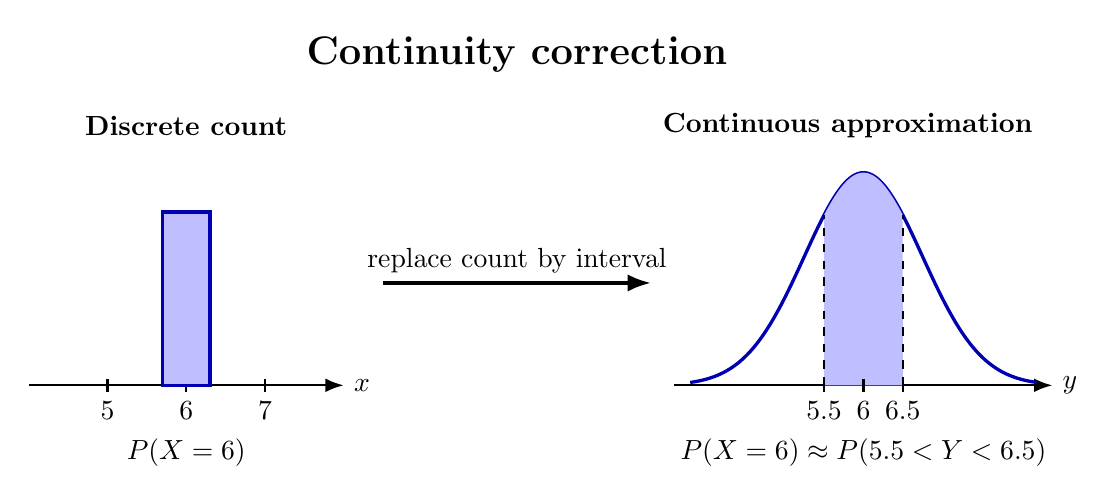
\begin{tikzpicture}[x=1cm,y=1cm,>=Latex]
\node[font=\Large\bfseries] at (0,4.2) {Continuity correction};
\node[font=\bfseries] at (-4.2,3.3) {Discrete count};
\draw[->, thick] (-6.2,0) -- (-2.2,0) node[right] {$x$};
\foreach \x/\lab in {-5.2/5,-4.2/6,-3.2/7}{\draw[thick] (\x,0.08) -- (\x,-0.08);\node[below] at (\x,-0.08) {$\lab$};}
\fill[blue!25] (-4.5,0) rectangle (-3.9,2.2);
\draw[blue!70!black, very thick] (-4.5,0) rectangle (-3.9,2.2);
\node[align=center] at (-4.2,-0.85) {$P(X=6)$};
\draw[->, very thick] (-1.7,1.3) -- (1.7,1.3);
\node[above] at (0,1.3) {replace count by interval};
\node[font=\bfseries] at (4.2,3.3) {Continuous approximation};
\draw[->, thick] (2.0,0) -- (6.8,0) node[right] {$y$};
\draw[very thick, blue!70!black, domain=2.2:6.6, samples=200] plot (\x,{2.7*exp(-0.5*((\x-4.4)/0.75)^2)});
\fill[blue!25, domain=3.9:4.9, samples=120] plot (\x,{2.7*exp(-0.5*((\x-4.4)/0.75)^2)}) -- (4.9,0) -- (3.9,0) -- cycle;
\draw[dashed, thick] (3.9,0) -- (3.9,{2.7*exp(-0.5*((3.9-4.4)/0.75)^2)});
\draw[dashed, thick] (4.9,0) -- (4.9,{2.7*exp(-0.5*((4.9-4.4)/0.75)^2)});
\foreach \x/\lab in {3.9/5.5,4.4/6,4.9/6.5}{\draw[thick] (\x,0.08) -- (\x,-0.08);\node[below] at (\x,-0.08) {$\lab$};}
\node[align=center] at (4.4,-0.85) {$P(X=6)\approx P(5.5<Y<6.5)$};
\end{tikzpicture}
\end{document}
